\chapter{Matematický popis implementovaných algoritmov}
V tejto kapitole je analýza existujúcich algoritmov pre fuzzifikáciu numerických hodnôt




\section{Algoritmus 1.  Fuzzifikácia založená na fuzzy entropii } 

Táto sekcia popisuje fuzzy klasifikátor založený na meraní fuzzy entropie s možnosťou výberu vlastností (FEBFC).

\subsection{Fuzzy klasifikátor založený na fuzzy entropii}
Fuzzy entropia je použitá na vyhodnotenie informácie o distribúcii vzorov v priestore vzorov. S touto informáciou vedia rozdeliť priestor vzorov na disjunktné rozhodovacie oblasti pre rozoznávanie vzorov. Vďaka tomu, že rozhodovacie oblasti sú disjunktné, aj komplexnosť, aj výpočtová náročnosť je zredukovaná. Tým pádom aj čas trénovania a klasifikácie je extrémne krátka. Hoci rozhodovacie oblasti sú rozdelené do disjunktných pod priestorov, môžu dosiahnuť kvalitnú klasifikáciu vďaka tomu, že pod priestory boli správne stanovené navrhovaným meraním fuzzy entropie. Okrem toho sa skúma ďalšie využitie fuzzy entropie na vybraté prvky. Procedúra výberu prvkov nielenže znižuje dimenziu problému, ale aj redukuje šum, zbytočné a nedôležité prvky.\cite{lee2001}


V klasifikačnom systéme je najdôležitejší postup rozdelenia priestoru vzoriek do rozhodovacích oblastí. Raz, keď je rozhodovacia oblasť určená, tak sa aplikujú na klasifikáciu neznámych vzorov.  Rozdelenie do rozhodovacích oblastí je súčasťou je súčasťou procesu učenia či tréningového procesu, pokiaľ rozhodovacie oblastí sú rozdelené tréningovými vzormi. 

V fuzzy klasifikátore založenom na fuzzy entropii sú rozhodovacie oblasti uzavreté od povrchov vytváraných z každého rozmeru. Povrchy sú určené rozložením vstupných dát.  
Pri vytváraní intervalov pre každý rozmer, alebo ekvivalentne, sa musí vygenerovať niekoľko trojuholníkových funkcií príslušnosti pre každú reálnu hodnotu atribútu (tento proces sa nazýva diskretizácia atribútov).  \cite{lee2001}
Počet intervalov na každom rozmere musí byť určený, ako aj centrum a šírka na každom intervale.  Metóda využíva fuzzy entropiu na určenie vhodného počtu intervalov. Používa k-means algoritmus na určenie stredu intervalov. Potom ako sú určené centrá intervalov je jednoduché rozhodnúť o šírke každého intervalu.
\paragraph*{} Z vyššie uvedeného popisu je možné zhrnúť Algoritmus 1. na  nasledujúce štyri kroky:

\begin{description}
\item[Krok A.] Určenie počtu intervalov na každý rozmer.
\item[Krok B.] Určenie polohy intervalu, t.j. určenie centra a šírku pre každý interval.
\item[Krok C.] Priradenie funkcie príslušnosti pre každý interval.
\item[Krok D.] Označenie tried pre každú rozhodovaciu oblasť.

\end{description}

\paragraph*{}
Podrobnejší popis jednotlivých krokov je popísaný v nasledujúcej časti. 

\subsection{Určenie počtu intervalov}
Počet intervalov v každom rozmere má zásadný vplyv na určenie účinnosti a presnosti klasifikácie. Ak je počet intervalov príliš veľký, tak bude dlho trvať pokým sa skončí tréningový a klasifikačný proces, a môže nastať pretečenie. 
Na druhú stranu, ak je počet intervalov malý, tak veľkosť každej rozhodovacej oblasti môže byť veľmi veľká, aby sa zmestila do rozdelenia vstupných vzorov, a výkon klasifikácie sa môže spomaliť. \cite{lee2001}

Kroky na zvolenie vhodného počtu intervalov pre každý rozmer sú: 
\begin{description}
\item[Krok A.1] Nastavenie počiatočného počtu intervalov \textit{I = 2}.
\item[Krok A.2] Nájdenie centier intervalov. 
\item[Krok A.3] Priradenie funkcie príslušnosti pre každý interval. 
\item[Krok A.4] Vypočítanie celkovej fuzzy entropie pre všetky intervaly \textit{I} a \textit{I-1}. 
Počíta sa fuzzy entropia na všetkých intervalov, aby sa získala informácia o rozložení vzorov v tejto dimenzii.
\item[Krok A.5] Klesla celková fuzzy entropia? 
V prípade, že celková fuzzy entropia na intervale I je menšia ako na intervaloch \textit{I-1}, tak sa znova rozdelia \textit{(I = I + 1)} a prejde sa na Krok A.2, inak sa prejde na Krok A.6. 
\item[Krok A.6]\textit{ I-1} je počet intervalov na zadanom rozmere. 
Vzhľadom na to, že fuzzy entropia neklesá, tak sa zastavilo ďalšie delenie na tejto dimenzii a \textit{I-1} je počet intervalov na danom rozmere.   
\end{description}

\subsection{Určenie polohy intervalov}

Proces určenia polohy intervalov začína s nájdením stredových bodov pre každý interval. Na nájdenie centier je použitý algoritmus \cite{chi36, duda37}. 
Predpokladajme, že je \textit{N} počet \textit{M}-rozmerných vektorov $V_i=(v_{i1}, v_{i2},…, v_{iM} )^T, i = 1, 2, \ldots, N$, čo zodpovedá \textit{N} prvkov. Pre rozdelenie prvkov do niekoľkých intervalov v rozmere \textit{j}, sa najprv vyberie \textit{N} hodnôt z prvkov reprezentujúcich tento rozmer $x_i^{(j)} = v_{ij}$. K-means zhlukovací algoritmus je použitý na klasterizáciu $x_i^{(j)} = v_{ij}.$ \cite{lee2001}
\paragraph{}
Algoritmus určenia polohy intervaly pozostáva z nasledujúcich krokov: 
\begin{description}
\item[Krok B.1] Nastavnie inicializačného počtu zhlukov \textit{I}. 
\item[Krok B.2] Určenie počiatočných stredov klastrov. 


Počiatočné centrá klastrov $c_1, c_2, \ldots, c_I$ môžu byť náhodne vybrané z $x_i^{(j)} = v_{i j}.$ Centrá klustrov $c_q$ ľubovolného klastra\textit{ q} sú priradené nasledovne: 
$$ c_q = \frac{q-1}{I-1},  q = 1, 2, \ldots, I.  $$
\item[Krok B.3] Priradenie označenia klastra pre každý element. 


Po určení klastrových centier,  sa priradí označenie pre každý prvok klastra podľa ktorého stred klastra je najbližšie. Toto je centrum s najmenšou eklidovskou vzdialenosťou od prvku. To znamená, že najbližšie centrum spĺňa nasledujúce meranie vzdialenosti: 
$$\left| {x_i^{(j)} – c_q^*} \right|  = \min\limits_{1 \leq q \leq I}  \left| {x_i^{(j)} –  c_q} \right|  $$
kde $c_q^*$ je najbližší stred k prvku $x_i^{j}$, teda medzi $c_1, c_2, \ldots,  c_I, c_q^*$ má najmenšiu euklidovskú vzdialenosť ku $x_i^{(j)}$.

\item[Krok B.4]Prepočítanie klastrových centier.

 
Vzhľadom na to, že počiatočné centra sú vybrané náhode, tak sa musí prepočítať  každé centrum nasledujúcim spôsobom: 

 $$c_q=\frac{\sum\limits_{q=1}^{N_q} x_i^{(j)} }{N_q}, $$
kde $N_q$ je celkový počet vzorov v rovnakom zhluku \textit{q}. 

\item[Krok B.5] Zmenil sa nejaký stred? 

Ak každý stred zhluku je vhodne určený,tak potom prepočítanie centier v Kroku B.4 to nezmení. Ak áno, zastaví sa určovanie centier intervalov, inak sa prejde na Krok B.3 \cite{lee2001}.
\end{description}


\subsection{Priradenie funkcie príslušnosti pre každý interval}

Priradenie funkcie príslušnosti je procedúra pre priraďovanie funkcie príslušnosti pre každý interval. Na aplikovanie fuzzy entropie sa zhodnotí informácia rozdelenia vzoru v danom intervaly. Priradí sa zhodná funkcia príslušnosti pre každý interval, aby indikovala stupeň príslušnosti prvku. Hodnota v intervale môže byť videná ako stupeň elementu patriaci tomu intervalu. Intervalový stred má najvyššiu hodnotu príslušnosti, ak hodnota príslušnosti prvku klesá ako vzdialenosť medzi týmito elementami a súhlasný interval centra sa zvyšuje.Preto sa priradí najvyššia hodnota príslušnosti 1 centru intervalu, a najnižšia hodnota 0 susedom centra tohto intervalu. V tomto variante sa využíva trojuholníková fuzzy množina. Na obrázku č. \ref{fig:prikladFunkciePrislusnosti} sa predpokladá, že $c_1, c_2, c_3, c_4$ sú centrá intervalov. Hodnoty všetkých elementov sú normalizované pre interval \textit{[0, 1]} pre jednoduchosť. \cite{lee2001}

Pri priraďovaní funkcie príslušnosti intervalu, tak sa zhodnocujú tieto tri prípady: 

\begin{description}
\item[Najľavejší interval] 

V tomto prípade, ako je ukázané na obrázku č. \ref{fig:prikladFunkciePrislusnosti}, prvý centrum intervalu $c_1$ na tomto rozmere je ohraničený len jedným intervalovým centrom $c_2$. Najvyššia hodnota príslušnosti 1 tohto intervalu sa nachádza v $c_1$, kde je najnižšia hodnota príslušnosti 0 je v $c_2$. Keď $x=0$, hodnota príslušnosti je určená ako 0.5, ako je ukázané na obrázku č. \ref{fig:prikladFunkciePrislusnosti}. Funkcia príslušnosti $\mu_{i1}$ najľavejšieho intervalu na rozmere \textit{i} je definovaná nasledovne:  

$$
\mu_{i, 1}(x) = 
\begin{cases}
{\frac{c_1 + x}{2c_1}, } &  \textrm{pre } x \leq   c_1 ,
\\
\max\left\{1 -\frac{| x-c_1|}{ | c_2 - c_1 |} \right\},
&  \textrm{pre } x >  c_1, \end{cases}
$$

kde $c_1$ je centrum najľavejšieho intervalu, a $c_2$ je centrum prvého centra intervalu vpravo od $c_1$. 

\item[Najpravejší interval ]
V tomto prípade, ako je ukázané na obrázku  č. \ref{fig:prikladFunkciePrislusnosti}, funkcia príslušnosti $\mu_{i4}$ najpravejšieho intervalu na rozmere i je definovaný nasledovne:

\begin{displaymath}
\mu_{i, 4}(x) = 
\begin{cases} 
\max \left\{
1 -\frac{| c_4-x|}{c_4-c_3} , 0
\right\}, 
& \textrm{pre } x \leq   c_4 ,
\\ 
\frac{2- x - c_4 }{2(1-c_4)}, 
& \textrm{pre } x >   c_4 ,
  \end{cases}, 
\end{displaymath}

kde $c_4$ je centrom najpravejšieho intervalu, a $c_3$ je centrom prvého intervalu vľavo od $c_4$. 


\item[Interný interval]
V tomto prípade, ako je ukázané na obrázku  č. \ref{fig:prikladFunkciePrislusnosti}, center $c_3$ interného intervalu je ohraničený jeho ľavým intervalovým centrom $c_2$ a pravým intervalovým centrom $c_4$. Najvyššia hodnota príslušnosti sa nachádza v $c_3$, a najnižšie hodnoty sú v centrách $c_2$ a $c_4$. Funkcia príslušnosti $\mu_{i3}$ je tretím intervalom v rozmere \textit{i} v tomto prípade definovanom ako  
$$
\mu_{i, 3}(x) = 
\begin{cases}
\max \left\{
1 -\frac{| c_3-x|}{|c_3-c_2|} , 0
\right\}, 
& \textrm{pre } x \leq   c_3,
\\
\max \left\{
1 -\frac{| c_3-x|}{|c_4-c_3|} , 0
\right\}, 
& \textrm{pre } x >  c_3.
\end{cases} 
$$

\end{description}

\begin{figure}[h]
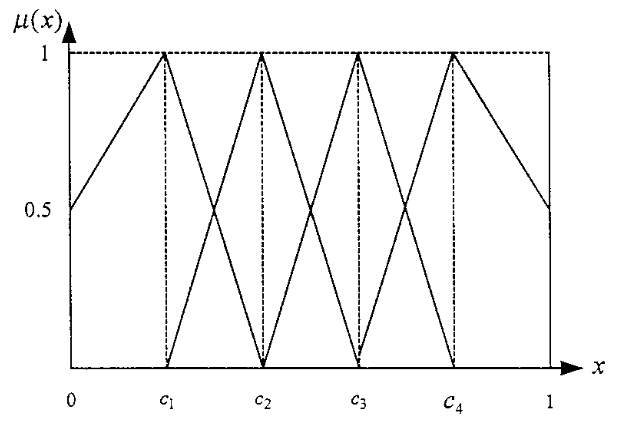
\includegraphics[width=0.75\textwidth]{obrazky/prikladFunkciePrislusnosti4}
\centering
\caption{Príklad priradenia funkcie príslušnosti pre intervalové centrá $c_1, c_2, c_3, c_4$ a trojuholníky korešpondujúce s funkciou príslušnosti\cite{lee2001}.} 
\label{fig:prikladFunkciePrislusnosti}
\end{figure}

\subsection{Označenie tried pre každú rozhodovaciu oblasť}
 V tomto kroku sa vypočíta fuzzy entropia pre každú vlastnosť cez sumarizáciu fuzzy entropie vo všetkých intervalov v tomto rozmere vlastnosti.
 
 Pre označenie tried v každej rozhodovacej oblastí sa musí použiť metóda na určenie fuzzy entropie. Fuzzy entropia rozhodovacích oblastí pre vzory každej triedy sú počítané tak, aby sa určila trieda pre každú rozhodovaciu oblasť. Fuzzy entropia rozhodovacích oblastí môže byť získaná cez sumarizáciu fuzzy entropie individuálnych intervalov pre každú vlastnosť rozmeru. Triede sa priradia rozhodovacia oblasť s najnižšou fuzzy entropiou v tejto oblasti.  Raz keď je rozhodovacia oblasť priradená a trieda označená, tak trénovanie je kompletné\cite{lee2001}.

\subsection{Výber vlastností}
Nový prístup pre výber funkcie založenej na fuzzy entropii je popísaný v nasledujúcom odseku.

 Fuzzy entropia odráža viac informácií v aktuálnom rozložení vzorov v priestore vzoriek. Vzhľadom k tomu, že fuzzy entropia je schopná rozlíšiť rozdelenie vzorov lepšie, používa sa na hodnotenie oddeliteľnosti jednotlivých funkcií.  Intuitívne, keď je nižšia fuzzy entropia vlastností, tak tým vyššie je znevýhodnenie vlastností.\cite{lee2001}.

Akonáhle je určená fuzzy entropia pre každú vlasnosť, tak sa môžu vyberať vlastností podľa výberu dopredu (\textit{forward selection}) alebo dozadu (\textit{backward elimination}). Metóda výberu dopredu je určenie relevantných vlastností na začiatku s prázdnou množinou a iteratívne pridávať vlastností až pokým nie sú splnené kritérium na zastavenie. Na rozdiel od toho eliminačná metóda vzad začína so všetkými vlastnosťami v množine, a odstraňuje vlastností pokým sú splnené kritérium na zastavenie.  
V Algoritme 1. sa používa eliminačná metóda vzad na selektovanie relevantných vlastností.  Kritérium zastavenia v tejto metóde je založená na klasifikácii rýchlosti triediča  Vzhľadom k tomu, že vlastností s vyššou fuzzy entropiou sú málo relevantné pre klasifikačný cieľ, tak sa odstránia vlastnosti ktoré majú najvyššiu fuzzy entropiu, ak to nezníži mieru klasifikácie. Potom sa opakuje vyššie spomenutý krok až pokým všetky irelevantné vlastností sú odstránené. Napokon ľavé vlastností sú určené ako vlastností pre klasifikáciu. S touto selekciou vlastností sa môže znížiť problém s rozmerom, aby sa urýchlil proces klasifikácie. V niektorých prípadoch sa môžu dosadnúť lepšie výsledky klasifikácie tým, že odhalíme nadbytočné, šumivé alebo nedôležité vlastnosti\cite{lee2001}.
\subsection{Zhrnutie Algoritmu 1. }
Cieľom tradičnej klasifikácie vzorov je rozdelenie priestoru vzoriek do rozhodovacích oblastí a to jednu oblasť pre každú triedu. V mnohých klasifikačných systémoch sú práve rozhodovacie oblasti  rozdelené do prekrývajúcich sa oblastí. Hoci klasifikátor s prekrývajúcimi rozhodovacími oblastiami môže dosiahnúť lepšiu klasifikačnú výkonnosť, ale to trvá dlhšie pre uzatvorenie rozhodovacích oblastí\cite{lee2001}.

Táto metóda je prezentovaná ako efektívny klasifikátor s výberom vlastností založený na fuzzy entropii pre klasifikáciu vzoru. Vzorový priestor je rozdelený do neprekrývajúcich fuzzy rozhodovacích oblastí. Vzhľadom na to, že rozhodovacie oblastí sú fuzzy pod-oblasti, tak sa môžu získať hladké hranice, pre dosiahnutie lepšieho výkonu klasifikácie. Aj keď rozhodovacie oblastí sa neprekrývajú, tak môžu znížiť výpočtovú zložitosť a záťaž klasifikátora\cite{lee2001}.

Tiež sa používa fuzzy entropia na vybranie relevantných vlastností. Aplikovanie výberu vlastností nielen zníži problém s rozmerom, ale ako aj zlepší výkonnosť klasifikácie odstránením zbytočných, šumivých, nedôležitých vlastností. Taktiež algoritmus K-means zhlukovania bol použitý na určenie funkcie príslušnosti pre každú vlasnosť\cite{lee2001}.





\subsection{Algoritmus 2. Modifikácia - Hierarchická fuzzy entropia}
%(FC-HFE)
Táto sekcia popisuje fuzzy klasifikátor založený na hierarchickej fuzzy entropii (FC-HFE), ktorý vychádza z Algoritmu 1. 


Algoritmus 1. má nasledovné problémy: 
\begin{itemize}
	\item Označovanie tried pre každú rozhodovaciu oblasť.	
	\item Rastúci počet intervalov na každej dimenzii.	
	\item Neprekrývajúce sa rozhodovacie oblasti. 
\end{itemize}



Označovanie tried pre každú rozhodovaciu oblasť je vykonávané podľa fuzzy entropie súčtom individuálnych intervalov pre každú dimenziu. Rozhodovacia oblasť je priradená triede s najnižšou fuzzy entropiou v danej oblasti. Podľa axiómu fuzzy entropie, fuzzy entropia bude nula, napriek tomu či  stupeň príslušnosti bude  pre každú triedu nula alebo jedna. Priraďovanie tried bude mať chyby, keď počet tried v ktorých fuzzy entropia sa rovná nule je viac ako jeden v tejto oblasti\cite{cheng2006}.

Rastúci počet intervalov na každej dimenzii je vykonaný podľa pravidla,pre ktoré celková entropia \textit{I }intervalov je menej ako to pre \textit{I-1} intervalov. Niekedy práve toto pravidlo zabraňuje v raste počtu intervalov, ktoré vedie k nesprávnej klasifikácii. Napríklad, dáta sú prezentované ako párne pretínajúce rozdelenie, napríklad dáta tvaru špirály.  Fuzzy entropia špirálových dát tohto typu je na začiatku vysoká, dáta by mali byť neskôr rozdelené na základe klesajúcej fuzzy entropie. Preto podmienka na zastavenie algoritmu pre rastúci počet intervalov bude výsledok v obmedzení rastúceho počtu intervalov na každej dimenzii\cite{cheng2006}.

Vzorový priestor bol rozdelený do neprekrývajúcich sa rozhodovacích oblastí použitím mriežkového rozdelenia. Označovanie tried nemôže byť priradené do rozhodovacej oblasti, ktorá nemá žiadne trénovacie dáta. Ak testovacia vzorka padá do danej rozhodovacej oblasti, ktoré systém nevie ako klasifikovať\cite{cheng2006}. 


Modifikácia upravuje pôvodný algoritmus v určovaní počtu intervalov napríklad udržiava pôvodnú podmienku pre zastavenie rastu počtu intervalov, ak celková entropia \textit{I} intervalov je viac ako jeden z \textit{I-1} intervalov. Ďalšia podmienka pre zastavenie rastu počtu intervalov je, ak celková fuzzy entropia \textit{I} intervalov je viac ako jedna z \textit{I-1} intervalov a celková fuzzy entropia \textit{I-1} intervalov je menej ako prahová hodnota  $\varphi$. To je, keď celková fuzzy entropia \textit{I} intervalov je menšia ako jedna z \textit{I-1} intervalov. Alebo celková entropia \textit{\textit{I}} intervalov je viac ako prahová hodnota $\varphi$, tak $I=I+1$. 

Hodnota prahovej hodnoty $\varphi$ bola vypočítaná použitím nasledovnej rovnice:

$$\varphi= -N_{trieda} \ast \frac{1}{N_{trieda}} \ast \log_2{(\frac{1}{N_{trieda}})}\ast (I-1) \ast \theta = - \log_2{(\frac{1}{N_{trieda}})} \ast (I-1) \ast \theta$$


kde $N_{trieda}$ je počet tried s hodnotami, a $\theta$ je percento maximálnej celkovej fuzzy entropie z \textit{I-1} intervalov. $\theta$ môže byť ladený použitím odlišného klasifikačného problému. Preto, môžu produkovať dostatok intervalov pre rovnomerné preniky dáta distribúcii použitím tejto metódy. Fuzzy entropia pre každú dimenziu musí byť menej ako špecifická hodnota. 

Ďalší fenomén je hodnota fuzzy entropie pre niektoré rozhodovacie oblasti je vždy veľmi vysoká. Rozdelenie dát rozhodujúcej oblasti je veľmi nejednoznačné alebo dáta je veľmi veľa nesprávne klasifikované dát.  Vzorkový priestor je rozdelený do toľko rozhodovacích oblastí fuzzy entropiou, zabraňujúc narastaniu klasifikačnej hodnote. 

Modifikácia sa zaoberá vyššou fuzzy entropiou rozhodovacích oblastí nazývaných hierarchická fuzzy entropia.  Štruktúra je zobrazená na obrázku \ref{fig:decisionRegions}. 2D vzorkový priestor na obrázku \ref{fig:decisionRegions} je rozdelený do nerovnomerných 53 rozhodovacích oblastí hierarchickou fuzzy entropiou. Prvá až štvrtá rozhodovacia oblasť fuzzy entropie vrstvy \textit{I} je veľmi vysoká. Rozdelili sa tieto rozhodovacie oblasti. Napríklad rozhodovacia oblasť \textit{I} bola rozdelená do ôsmych rozhodovacích oblastí po druhý raz. Rozhodovacie pod oblasti \textit{I} a \textit{II} boli rozdelené do štyroch rozhodovacích oblastí retrospektívne po tretí raz. Rozhodovacie oblasti \textit{I} boli rozdelene do štrnástich rozhodovacích oblastí. Fuzzy entropia väčšiny rozhodovacích oblastí sa stala nižšou po tom, ako bol vzorkový priestor rozdelený použitím hierarchickej fuzzy entropie. \cite{cheng2006}.


\begin{figure}[h]
	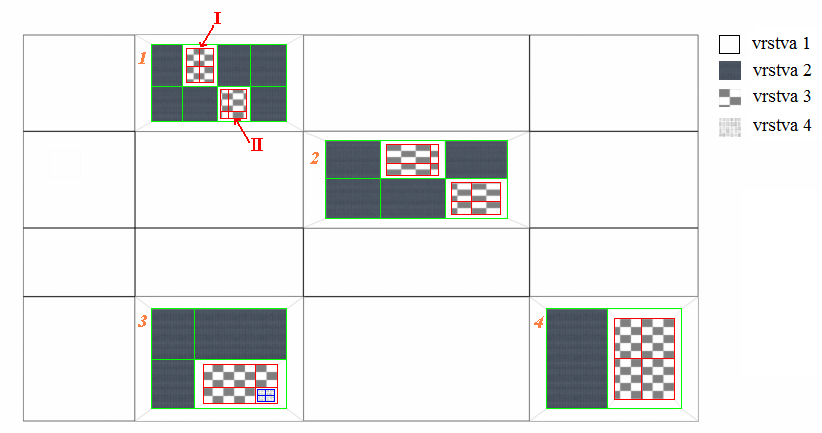
\includegraphics[width=0.75\textwidth]{obrazky/decisionRegions}
	\centering
	\caption{Pohľad zhora na rozdelené rozhodovacie oblasti použitím hierarchickej entropie \cite{cheng2006}.} 
	\label{fig:decisionRegions}
\end{figure}



Okrem toho, je  modifikovaná metóda, ktorou sa počíta fuzzy entropia pre rozhodovacie oblasti. Ak tam nie sú žiadne trénovacie dáta určitej triedy na intervale, tak množina fuzzy entropie tejto triedy sa rovná jednej. To je preto, aby sa zabránilo tomu, že fuzzy entropia určitej triedy sa bude rovnať nule viac ako jedenkrát pre počítanie najnižšej fuzzy entropie oblasti. 


{Algoritmus 2.} má tieto nasledujúce kroky \cite{cheng2006}.: 


\begin{description}
\item[Krok 1 – Krok 4.] je rovnaký ako v Algoritme 1. v selektovaní počtu intervalov pre každú dimenziu na aktuálnom vzorovom priestore. 

\item[Krok 5.] Ak celková fuzzy entropia I intervalu je menej ako I-1 intervalu alebo celková fuzzy entropia \textit{I} intervalu je viac ako prahová hodnota $\varphi$, tak sa znova rozdeľuje $(I = I - 1)$ a ide na krok 2. Inak sa zastaví zvyšovanie intervalov na tejto dimenzii a rozhodne sa počet intervalov pre ďalšiu dimenziu. 
			
\item[Krok 6.] Akonáhle  pre každú dimenziu sú intervaly určené, rozhodovacie oblasti pre súčasný vzorkový priestor sú rozdelené.  Stredná hodnota fuzzy entropie je vypočítaná použitím nasledujúcej rovnice pre všetky rozhodovacie oblasti: 
$$MFE_i =  \frac{\sum\limits_{i=1}^{N_i}FE_{ij}}{ N_i},  j=1 \dots N_i, $$
kde $N_i$ je počet rozhodovacích oblastí pre \textit{i}-tú vrstvu, $FE_{ij}$ je \textit{j}-tá rozhodovacia oblasť pre \textit{i}-tú vrstvu a $MFE_i$ je stredná hodnota fuzzy entropie pre \textit{i}-tú vrstvu. 
				
\item[Krok 7.] Fuzzy entropia pre každú rozhodovaciu oblasť v súčasnom vzorovom priestore je porovnávaná s \textit{MFE}. Ak fuzzy entropia pre rozhodovaciu oblasť je väčšia ako stredná hodnota fuzzy entropie, oblasť sa stane nezávislým pod priestorom a Krok 1. až Krok 7. sú vykonávané znova na určenie rozhodovacích oblastí pre každý pod priestor.  Inak rozhodovacia oblasť bude pridelená označeniu triedy. 

\end{description}

Horeuvedené kroky sú ako rekurzívna funkcia, ktorá je vykonávaná opakovane pre každý pod priestor až pokiaľ všetky pod priestory nemôžu byť viac rozdelené. Keď kroky sú skončené, testovací vzor je klasifikovaní použitím rozhodovacích oblasti, ktorá majú označenie triedy. Keď testovacia vzorka nemá označenie triedy oblasti triedy, tak testovacia vzorka je porovnávaná použitím krátkej euklidovskej vzdialenosti medzi susedmi trénovaných dát a testovacej vzorky, klasifikované do najbližšej trénovanej triedy.\cite{cheng2006}.



\subsection{Algoritmus 3. Modifikácia  - Vážená entropia }
Táto sekcia popisuje fuzzy klasifikátor založený na váženej entropie
Algoritmus 3. sa od Algoritmu 1. odlišuje v spôsobe výpočtu funkcie príslušnosti lingvistickej premennej, tak aby hodnota sumy hodnôt funkcie príslušnosti bola rovná jednej. Ďalej pri výbere kritéria efektívnosti rozkladu na intervaly v tvare váženej fuzzy entropie, ktorá berie do úvahy aj počet elementov patriacich do získaných intervalov. Základná myšlienka spočíva v postupnom rozklade množiny $X$ na $2,\ldots, n$ intervalov a kontrole efektívnosti tohto rozkladu.  \cite{levashenkoProj}

\subsubsection{Vstupné dáta}
Počet \textit{N} hodnôt vstupného atribútu, zadaného množinou reálnych čísel $X={x_1, \ldots,x_i, \ldots, x_N}$. 
Počet K možných hodnôt výstupného atribútu $B={b_1, \ldots, b_k, \ldots, b_K}$, ku ktorým patria prvky množiny \textit{X}. Množina dvojíc $(x_i, b_k)$ definuje  vzťah medzi každou hodnotou množiny \textit{X} a hodnotou výstupného atribútu. \cite{levashenkoProj}

\subsubsection{Výstupné dáta}
Počet \textit{Q} intervalov, na ktoré je potrebné rozložiť vstupnú množinu reálnych čísel \textit{X} (počet termov lingvistickej premennej). Matica príslušnosti \textit{U} s rozmermi $N \times Q$. \cite{levashenkoProj}

\subsubsection{Kroky algoritmu}
Algoritmus 4. sa skladá z týchto ôsmych krokov:  



\begin{description}
\item[{Krok 1.}]   Určenie počiatočného počtu intervalov Q = 2. 
\item[{Krok 2.}] Vybratie náhodného počiatočného centra každého intervalu $ I = \left\{C_1, \ldots, C_Q\right\}$. 

 \item[{Krok 3.}]  Určenie intervalu, kde patrí každý element $x_i$. Kritérium je najmenšia hodnota euklidovskej vzdialenosti.

  \item[{Krok 4.}]
  Nové centrá \textit{I} sú určené pre každý interval ako aritmetický priemer hodnôt prvkov $x_i$, patriacich do týchto intervalov
  $$
  C_q = \frac{ \sum\limits_{i=1}^{N_q} x_i }{N_q} , 
  $$
  kde $N_q$ je počet prvkov $x_i$ patriacich do intervalu $C_q$.  
   \item[{Krok 5.}] Ak sa jedno z vypočítaných nových centrier zmenilo, tak sa pokračuje Krokom 3, v opačnom prípade Krokom 6. 
   
   
    \item[{Krok 6.}] Definícia funkcii príslušnosti lingvistickej premennej pre každý z \textit{Q} termov. Získaný výsledok predstavuje hľadanú maticu príslušnosti \textbf{U}. 
    
    
\item[{Krok 7.}] 
 Vypočítanie váženej fuzzy entropie $wFE(A)_Q$ pri rozklade na \textit{Q} intervalov. 
 
 \item[{Krok 8.}] 
 Vypočítaná fuzzy entropia $wFE(A)_Q$  sa porovná s predchádzajúcou hodnotou $wFE(A)_{Q-1}$ . Pričom prvá hodnota je veľké číslo $wFE(A)_1=+\infty$. 
 V prípade, že táto entropia neklesá, tak sa zväčší počet intervalov $Q=Q+1$ a zopakujú sa všetky výpočty vrátane Kroku 2. 
 V opačnom prípade hodnota \textit{$(Q-1)$} je optimálny počet intervalov. \cite{levashenkoProj}
\end{description}


\section{Algoritmus 3. Modifikácia s Fuzzy k-means algoritmom}

Táto modifikácia namiesto klasického k-meansu algoritmu použije FCM algoritmus na určenie polôh centier v intervaloch. 

Výhody FCM algoritmu sú, že dáva najlepšie výsledky pre prekrývajúce sa súbory dát a pomerne lepšie ako k-means algoritmus.  Na rozdiel od k-means, kde dátový bod musí výlučne patriť do jedného centra klastra, v tomto dátovom bode je priradené členstvo v každom klastrovom centre, v dôsledku čoho môže byť dátový bod patriť do viac ako jedného centra klastra.

Nevýhody sú, že apriori sa definuje počt zhlukov. S nižšou hodnotou beta hodnoty dostaneme lepší výsledok, ale na úkor väčšieho početu iterácií. Euklidovské meranie vzdialenosti môže nerovnomerne zaťažiť základné faktory.

% * <chovancova@mail.com> 2017-04-19T18:20:08.910Z:
% 
% > Advantages
% > 1) Gives best result for overlapped data set and comparatively better then k-means algorithm.
% > 2) Unlike k-means where data point must exclusively belong to one cluster center here data point is assigned 
% >     membership to each cluster center as a result of which data point may belong to more then one cluster center.
% > Disadvantages
% > 1) Apriori specification of the number of clusters.
% > 2) With lower value of  β we get the better result but at the expense of  more number of iteration.
% > 3) Euclidean distance measures can unequally weight underlying factors.
% 
% ^.




%https://www.mathworks.com/help/pdf_doc/fuzzy/fuzzy.pdf
Fuzzy k-means (FCM) je metóda, ktorá umožňuje zhlukovanie pre každý dátovy bod, ktorý môže patriť do viacerým klastrov s rôznymi stupňami príslušnosti. 
\cite{Bezdec1981}

FCM metóda je založená na minimalizácii účelovej funkcie

$$J_m = \sum_{i=1}^{D}\sum_{j=1}^{N} { \mu_{ij}^m \left| \left| x_i - c_j \right|\right|^2  },$$ 
kde 
D je počet dátových bodov, N je počet klastrov, m je fuzzy časť exponentu matice pre riadenie stupňa fuzzy prekrytia,  m $>$ 1. 
Fuzzy prekrytie určuje ako rozmanité hranice sú medzi klastrami a aký počet dátových bodov majú významnú príslušnosť vo viac ako v jednom klastri. 
%fuzzy partition matrix exponent for controlling the degree of fuzzy overlap, with m > 1. 
Ďalej $x_i$ je i-tý dátový bod,  $c_j$ je centrum j-tého klastra, $\mu_{ij}$ je stupeň príslušnosti $x_i$ v j-tom klastri. \cite{fuzzyLogicToolbox}
 
Kroky Fuzzy k-means algoritmu : 
\paragraph{Krok 1.} Náhodne sa inicializujú klustre hodnoty príslušnosti, $\mu_{ij}$. 
\paragraph{Krok 2.} Vypočítanie centier klastra
$c_j = \frac{
\sum\limits_{i=1}^D \mu_{ij}^m  x_i 
}{
\sum\limits_{i=1}^D \mu_{ij}^m
}$

\paragraph{Krok 3.} Aktualizácia $\mu_{ij}$ podľa nasledujúceho vzťahu  
$\mu_{ij} = \frac{1}{\sum\limits_{k=1}^N  \left ( \frac {\left| \left| x_i - c_j \right|\right|}{\left| \left| x_i -c_k\right|\right|}\right) ^{\frac{2}{m-1}}}. $


\paragraph{Krok 4.} Vypočítanie účelovej funkcie $J_m$. 
\paragraph{Krok 5.} Opakovanie krokov 2-4 až pokým $J_m$ sa zlepší o menej než stanovená minimálna prahová hodnota alebo po uplynutí určitého maximálneho počtu iterácií. 



\section{Algoritmus 4. Vážená entropia s FCM algoritmom}

Kroky algoritmu sú tie isté ako v algoritme 1, ale pri podmienke na zastavenie sa bude brať vážená entropia. Na lokáciu centier intervalov sa použije FCM algoritmus.  

